\subsection{Post-inflationary inflaton dynamics and reheating (cap. 8)}

Cuando termina inflación tenemos que la energía cinética del campo inflatón se vuelve comparable con el valor de su potencial $(\dot{\phi}^2 \sim V(\phi))$ lo que implica que el parámetro de \textit{slow-roll} $\epsilon$ se acerca a $1$. En esta época dónde tenemos este régimen, el campo oscila alrededor de un mínimo del potencial.

A tiempos suficientemente grandes comparados con respecto al período de oscilación, podemos ignorar la expansión del universo para ver las oscilaciones éstas. Y a estas oscilaciones las llamaremos oscilaciones coherentes.

\subsubsection{Coherently oscillating scalar field}

Como durante estas oscilaciones coherentes vamos a despreciar la expansión del universo, entonces la densidad de energía del campo será de la forma

\begin{equation}
    \rho_\phi = \frac{1}{2} \dot{\phi}^2 + V(\phi) = V(\phi_0)
\end{equation}

\noindent
es decir, la consideramos como constante. Notemos que esta ecuación nos permite obtener la velocidad del inflatón en términos del potencial

\begin{equation}
    \dot{\phi} = \sqrt{2 \left[ V(\phi_0) - V(\phi) \right]}
\end{equation}

Para lo siguiente, planteemos un potencial monomial con $n > 0$ de la forma

\begin{equation}
    V (\phi) = V_0 \left( \frac{\phi}{m_p} \right)^{2n}
\end{equation}

\noindent
lo que implica que 

\begin{equation}
    \begin{split} 
        \dot{\phi} &= \sqrt{2 V (\phi_0) \left[ 1 - \frac{V(\phi)}{V(\phi_0)} \right]} = \sqrt{2 V(\phi_0)} \ \sqrt{1 - \left( \frac{\phi}{\phi_0} \right)^{2n}}
    \end{split}
\end{equation}

\paragraph{Time-averaged equation of state}

Para un modelo de un único campo escalar, la ecuación de estado está dada por

\begin{equation}
    \omega_\phi = \frac{P_\phi}{\rho_\phi} = \frac{\displaystyle \frac{1}{2} \dot{\phi}^2 - V(\phi)}{\displaystyle \frac{1}{2} \dot{\phi}^2 + V(\phi)}
\end{equation}

\noindent
podemos escribir ésto para el potencial monomial como

\begin{equation*}
    \begin{split}
        1 + \omega_\phi &= 1 + \frac{P_\phi}{\rho_\phi}\\
        1 + \omega_\phi &= \frac{P_\phi + \rho_\phi}{\rho_\phi}\\
        1 + \omega_\phi &= \frac{\displaystyle \frac{1}{2} \dot{\phi}^2 - V(\phi) + \frac{1}{2} \dot{\phi}^2 + V(\phi)}{\rho_\phi}\\
        1 + \omega_\phi &= \frac{\dot{\phi}^2}{\displaystyle \frac{1}{2} \dot{\phi}^2 + V(\phi)}\\
        1 + \omega_\phi &= \frac{2 \left[ V(\phi_0) - V(\phi) \right]}{V(\phi_0) - V(\phi) + V(\phi)}\\
        1 + \omega_\phi &= 2 \frac{V (\phi_0) - V(\phi)}{V(\phi_0)}\\
        1 + \omega_\phi &= 2 \left[ 1 - \frac{V(\phi)}{V(\phi_0)} \right]\\
        1 + \omega_\phi &= 2 \left[ 1 - \left( \frac{\phi}{\phi_0} \right)^{2n} \right] 
    \end{split}
\end{equation*}

\noindent
de acá podemos calcular el valor medio de $\omega_\phi$ sobre un período de oscilación y usemos el valor de $\dot{\phi}$ que obtuvimos para el potencial monomial junto con lo anterior

\begin{equation*}
    \begin{split}
        \langle 1 + \omega_\phi \rangle &= \frac{\displaystyle \int_0^{T_{osc}} (1 + \omega_\phi) \ dt}{\displaystyle \int_0^{T_{osc}} dt}\\
        1 + \langle \omega_\phi \rangle &= \frac{\displaystyle \int_0^{T_{osc}} (1 + \omega_\phi) \frac{dt}{d\phi} d\phi}{\displaystyle \int_0^{T_{osc}} \frac{dt}{d\phi} d\phi}\\
        1 + \langle \omega_\phi \rangle &= \frac{\displaystyle \int_0^{T_{osc}} \frac{1 + \omega_\phi}{\dot{\phi}} d\phi}{\displaystyle \int_0^{T_{osc}} \frac{1}{\dot{\phi}} d\phi}\\
        1 + \langle \omega_\phi \rangle &= \frac{\displaystyle \int_0^{T_{osc}} 2 \left[ 1 - \left( \frac{\phi}{\phi_0} \right)^{2n} \right] \left[ \colorcancel{red}{\sqrt{2 V(\phi_0)}} \sqrt{1 - \left( \frac{\phi}{\phi_0} \right)^{2n}} \right]^{-1} \ d\phi}{\displaystyle \int_0^{T_{osc}} \left[ \colorcancel{red}{\sqrt{2 V(\phi_0)}} \sqrt{1 - \left( \frac{\phi}{\phi_0} \right)^{2n}} \right]^{-1} \ d\phi}\\
        1 + \langle \omega_\phi \rangle &= \frac{\displaystyle \int_0^{T_{osc}} 2 \sqrt{1 - \left( \frac{\phi}{\phi_0} \right)^{2n}} \ d\phi}{\displaystyle \int_0^{T_{osc}} \left[ 1 - \left( \frac{\phi}{\phi_0} \right)^{2n} \right]^{-1/2} \ d\phi}
    \end{split}
\end{equation*}

\noindent
para estas integrales podemos usar los siguientes resultados:

\begin{equation}
    \int_0^1 \left( 1 - y^{2n} \right)^{1/2} \ dy = \frac{\displaystyle \Gamma \left( \frac{1}{2} \right) \ \Gamma \left( 1 + \frac{1}{2n} \right)}{\displaystyle 2 \Gamma \left( \frac{3}{2} + \frac{1}{2n}  \right)} \hspace{1.5cm} \int_0^1 \left( 1 - y^{2n} \right)^{-1/2} dy = \frac{\displaystyle \Gamma \left( \frac{1}{2} \right) \ \Gamma \left( 1 + \frac{1}{2n} \right)}{\displaystyle \Gamma \left( \frac{1}{2} + \frac{1}{2n} \right)}
\end{equation}

\noindent
entonces definamos como variable $\displaystyle y = \frac{\phi}{\phi_0}$ tal que la integral nos queda

\begin{equation*}
    \begin{split}
        1 + \langle \omega_\phi \rangle &= \frac{\displaystyle \phi_0 \int_0^1 2 \left( 1 - y^{2n} \right)^{1/2} \ dy}{\displaystyle \phi_0\int_0^1 \left( 1 - y^{2n} \right)^{-1/2} \ dy}\\
        1 + \langle \omega_\phi \rangle &= \frac{\displaystyle \colorcancel{red}{\Gamma \left( \frac{1}{2} \right)} \ \colorcancel{teal}{\Gamma \left( 1 + \frac{1}{2n} \right)}}{\displaystyle \Gamma \left( \frac{3}{2} + \frac{1}{2n} \right)} \cdot \left[ \frac{\displaystyle \colorcancel{red}{\Gamma \left( \frac{1}{2} \right)} \ \colorcancel{teal}{\Gamma \left( 1 + \frac{1}{2n} \right)}}{\displaystyle \Gamma \left( \frac{1}{2} + \frac{1}{2n} \right)} \right]^{-1}\\
        1 + \langle \omega_\phi \rangle &= \frac{\displaystyle \Gamma \left( \frac{1}{2} + \frac{1}{2n} \right)}{\displaystyle \Gamma \left( \frac{3}{2} + \frac{1}{2n} \right)}
    \end{split}
\end{equation*}

\noindent
puedo usar $\Gamma  (1 + z) = z \ \Gamma (z)$

\begin{equation*}
    \begin{split}
        1 + \langle \omega_\phi \rangle &= \frac{\displaystyle \Gamma \left( \frac{1}{2} + \frac{1}{2n} \right)}{\displaystyle \Gamma \left( 1 + \frac{1}{2} + \frac{1}{2n} \right)}\\
        1 + \langle \omega_\phi \rangle &= \frac{\displaystyle \colorcancel{red}{\Gamma \left( \frac{1}{2} + \frac{1}{2n} \right)}}{\displaystyle \colorcancel{red}{\Gamma \left( \frac{1}{2} + \frac{1}{2n} \right)} \cdot \left(\frac{1}{2} + \frac{1}{2n}\right)}\\
        1 + \langle \omega_\phi \rangle &= \frac{2n}{n + 1}\\
        \langle \omega_\phi \rangle &= \frac{2n}{n + 1} - 1
    \end{split}
\end{equation*}

\begin{equation}
    \langle \omega_\phi \rangle = \frac{n - 1}{n + 1}
\end{equation}

\noindent
notemos entonces que si tengo $n = 1$ tengo materia, si tengo $n = 2$ tengo radiación, para $n = 0$ tengo energía oscura y si $\displaystyle n < \frac{1}{2}$ tengo $\displaystyle \langle \omega_\phi \rangle < - \frac{1}{3}$ que nos da un universo en expansión.

\paragraph{Period of an anharmonic oscillator}

El período de oscilación del inflatón lo podemos calcular a partir de

\begin{equation}
    T_{osc} = \int_0^{T_{osc}} dt = 2 \int_{- \phi_0}^{\phi_0} \frac{d\phi}{\dot{\phi}}
\end{equation}

\noindent
desarrollemos esta expresión utilizando el valor que calculamos para $\dot{\phi}$ para un potencial monomial

\begin{equation*}
    \begin{split}
        T_{osc} &= 2 \int_{- \phi_0}^{\phi_0} \left\{ 2 V(\phi_0) \left[1 - \left(\frac{\phi}{\phi_0} \right)^{2n} \right] \right\}^{-1/2} \ d\phi\\
        &= \frac{2}{\sqrt{2 V(\phi_0)}} \int_{- \phi_0}^{\phi_0} \left[ 1 - \left( \frac{\phi}{\phi_0} \right)^{2n} \right]^{-1/2} \ d\phi
    \end{split}
\end{equation*}

\noindent
utilizo el cambio de variables $\displaystyle y = \frac{\phi}{\phi_0}$

\begin{equation*}
    \begin{split}
        T_{osc} &= \frac{2 \phi_0}{\sqrt{2 V(\phi_0)}} \int_{-1}^1 \left( 1 - y^{2n} \right)^{-1/2} \ dy\\
        &= \frac{4 \phi_0}{\sqrt{2 V(\phi_0)}} \int_0^1 \left( 1 - y^{2n} \right)^{- 1/2} \ dy\\
        &= \frac{4 \phi_0}{\sqrt{2 V(\phi_0)}} \frac{\displaystyle \Gamma \left( \frac{1}{2} \right) \ \Gamma \left( 1 + \frac{1}{2n} \right)}{\displaystyle \Gamma \left( \frac{1}{2} + \frac{1}{2n} \right)}\\
        &= \frac{4 \sqrt{\pi} \phi_0}{\sqrt{2 V(\phi_0)}} \frac{\displaystyle \Gamma \left( 1 + \frac{1}{2n} \right)}{\displaystyle \Gamma \left( \frac{1}{2} + \frac{1}{2n} \right)}
    \end{split}
\end{equation*}

\noindent
finalmente, escribamos de forma explícita el potencial $V(\phi_0)$

\begin{equation*}
    \begin{split}
        T_{osc} &= \frac{2 \sqrt{2 \pi} \phi_0}{\displaystyle \sqrt{V_0} \left( \frac{\phi_0}{m_p} \right)^n} \frac{\displaystyle \Gamma \left( 1 + \frac{1}{2n} \right)}{\displaystyle \Gamma \left( \frac{1}{2} + \frac{1}{2n} \right)}
    \end{split}
\end{equation*}

\begin{equation}
    T_{osc} = 2 \sqrt{2\pi} \frac{m_p}{\sqrt{V_0}} \frac{\displaystyle \Gamma \left( 1 + \frac{1}{2n} \right)}{\displaystyle \Gamma \left( \frac{1}{2} + \frac{1}{2n} \right)} \left( \frac{\phi_0}{m_p} \right)^{1 - n} 
\end{equation}

\noindent
podemos ver que para $n = 1$ (oscilador armónico), el período de oscilación es independiente de $\phi_0$ mientras que para $n > 1$ tenemos que los períodos decaen con $\phi_0$ y para $n < 1$ los periodos crecen con $\phi_0$.

\subsubsection{External coupling and decay of the inflaton condensate}

Si consideramos que el campo del inflatón está acoplado con otros campos tendremos que a medida que este campo decae su energía es transferida a los campos hijos que luego decaerán a otras partículas las cuales termalizarán con el resto del plasma primordial dando inicio a BBN. Por lo tanto, \textit{reheating} se supone que da comienzo al modelo de estándar que se conoce hoy en día, dando origen a las partículas calientes.

El decaimiento de este campo puede ser de naturaleza perturbativa como decaimiento del campo en partículas masivas, o de forma no perturbativa a través de mecanismos de resonancia paramétrica como consecuencia de las oscilaciones coherentes del campo. Cuál naturaleza es predominante depende de la aplitud de las oscilaciones del campo junto con la naturaleza del acople entre el inflatón y los grados de libertad de las partículas bosónicas y fermiónicas.

\paragraph{Perturbative reheating}

En el marco de la naturaleza perturbativa, el campo del inflatón podemos asumirlo como un gran número de partículas masivas de inflatón con poco momento, y cada partícula tiene una probabilidad de decaer en otras partículas de forma independiente. La probabilidad de decaer estará dada por $\Gamma$ y puede calcularse a partir de las reglas de Feynmann. Podemos agregar esta tasa de decaimiento en la ecuación de movimiento como un término de fricción de la forma

\begin{equation}
    \ddot{\phi} + (3H + \Gamma) \dot{\phi} + V_{,\phi} (\phi) =0
\end{equation}

Esta teoría funciona cuando el inflatón decae en fermiones $(\psi)$ a través de interacciones del tipo Yukawa $(h \psi \bar{\psi} \phi)$ con una constante de acople $h$ tal que $h^2 \ll \displaystyle \frac{m_\phi}{m_p}$ o cuando el inflatón está acoplado con un campo escalar bosónico $\chi$ a través de la interacción $\displaystyle \frac{1}{2} g^2 \chi^2 \phi^2$ haciendo que la producción de partículas por efectos no perturbativos como la resonancia paramétrica sea ineficiente.

Al principio de recalentamiento tenemos $H \gg \Gamma$, de otro modo la producción de partículas durante inflación modificaría el potencial del inflatón. Y el escenario perturbativo en recalentamiento termina cuando $H \simeq \Gamma$. Entonces la termalización de la temperatura de \textit{reheating} puede ser calculada a partir de 

\begin{equation*}
    \begin{split} 
        \Gamma &\simeq H\\
        \Gamma &= \sqrt{\frac{\rho (T_{re})}{3 m_p^2}}\\
        \Gamma &= \sqrt{\frac{\pi^2}{90} \frac{g_* (T_{re})}{m_p^2} \ T_{re}^4}\\
        T_{re}^4 &= \frac{90}{\pi^2} \frac{m_p^2 \Gamma^2}{g_* (T_{re})}\\
        T_{re} &= \left[ \frac{90}{g_* (T_{re})} \right]^{1/4} \sqrt{\frac{m_p \Gamma}{\pi}}
    \end{split}
\end{equation*}

\noindent
podemos notar que la temperatura de \textit{reheating} es independiente de la duración de inflación y de las propiedades del potencial del inflatón. Sin embargo, el acople entre el inflatón y los campos externos pueden alterar la forma del potencial en inflación a través de correcciones en los grados de libertad relativistas y estos pueden generar cotas en la tasa de decaimiento.

\paragraph{Non-perturbative reheating}

Para modelos inflacionarios en los que la fuente principal de recalentamiento es el decaimiento del inflatón en bosones tenemos que los efectos no perturbativos son importantes.

Nos enfocaremos en el escenario en el que el inflatón está acoplado a un campo escalar sin masa llamado $\chi$ a través de una interacción de la forma $\mathcal{I} (\phi, \chi)$ con un modelo que será descripto por la acción

\begin{equation}
    S [g_{\mu\nu}, \phi, \chi] = \int \sqrt{-g} \left[ \frac{m_p^2}{2} R - \frac{1}{2} \partial^\mu \phi \ \partial^\nu \phi \ g_{\mu \nu} - \frac{1}{2} \partial^\mu \chi \ \partial^\nu \chi \ g_{\mu \nu} - V(\phi) - \mathcal{I} (\phi, \chi) \right] d^4 x
\end{equation}

\noindent
a partir de esta acción podemos calcular las ecuaciones de movimiento a partir de las ecuaciones de Euler-Lagrange y usando que $g_{\mu \nu}$ es la métrica de FLRW

\begin{equation}
    \partial^\alpha \left[ \frac{\partial \mathcal{L}}{\partial (\partial_\alpha \varphi_k)} \right] - \frac{\partial \mathcal{L}}{\partial \varphi_k} = 0
\end{equation}

\noindent
con

\begin{equation*}
    \begin{split}
        \mathcal{L} &= \sqrt{-g} \left[ \frac{m_p^2}{2} R - \frac{1}{2} \partial_\mu \phi \ \partial_\nu \phi \ g^{\mu \nu} - \frac{1}{2} \partial_\mu \chi \ \partial_\nu \chi \ g^{\mu \nu} - V(\phi) - \mathcal{I} (\phi, \chi) \right]\\
        \mathcal{L} &= a^3 \left[ \frac{m_p^2}{2} R - \frac{1}{2} \left( - \partial_t \phi \ \partial_t \phi + \frac{1}{a^2} \partial_i \phi \ \partial_j \phi \ \delta_{ij} \right) - \frac{1}{2} \left( - \partial_t \chi \ \partial_t \chi + \frac{1}{a^2} \partial_i \chi \ \partial_j \chi \ \delta_{ij} \right) - V(\phi) - \mathcal{I} (\phi, \chi) \right]
    \end{split}
\end{equation*}

\noindent
ahora calculemos las ecuaciones de Euler-Lagrange para el campo $\phi$

\begin{equation*}
    \begin{split}
        \partial^t \left[ -\frac{a^3}{2} \left( - \partial_t \phi - \partial_t \phi \right) \right] + \partial^i \left[ -\frac{a}{2} \left( \partial_i \phi + \partial_i \phi \right) \right] + a^3 V_{, \phi} + a^3 \mathcal{I}_{,\phi} &= 0\\
        \partial^t (a^3 \partial_t \phi) - a \ \partial^i \partial_i \phi + a^3 V_{,\phi} + a^3 \mathcal{I}_{,\phi} &= 0\\
        3 a^2 \dot{a} \  \partial_t \phi + a^3 \partial^t \partial_t \phi - a \partial^i \partial_i \phi + a^3 V_{,\phi} + a^3 \mathcal{I}_{,\phi} &= 0\\
        3 \frac{\dot{a}}{a} \partial_t \phi + \partial^t \partial_t \phi - \frac{1}{a^2} \partial^i \partial_i \phi + V_{,\phi} + \mathcal{I}_{,\phi} &= 0
    \end{split}
\end{equation*}

\begin{equation}
    \ddot{\phi} - \frac{\nabla^2}{a^2} \phi + 3 H \dot{\phi} + V_{,\phi} + \mathcal{I}_{,\phi} = 0
\end{equation}

\noindent
hagamos lo mismo para $\chi$

\begin{equation*}
    \begin{split}
        \partial^t \left[ - \frac{a^3}{2} \left( - \partial_t \chi - \partial_t \chi \right) \right] + \partial^i \left[ - \frac{a}{2} \left(\partial_i \chi + \partial_i \chi \right) \right] + a^3 \mathcal{I}_{,\chi} &= 0\\
        \partial^t \left( a^3 \ \partial_t \chi \right) - a \partial^i \partial_i \chi + a^3 \mathcal{I}_{,\chi} &= 0\\
        3 a^2 \dot{a} \ \partial_t \chi + a^3 \ \partial^t \partial_t \chi - a \partial^i \partial_i \chi + a^3 \mathcal{I}_{,\chi} &= 0\\
        3 \frac{\dot{a}}{a} \partial_t \chi + \partial^t \partial_t \chi - \frac{1}{a^2} \partial^i \partial_i \chi + \mathcal{I}_{,\chi} &= 0
    \end{split}
\end{equation*}

\begin{equation}
    \ddot{\chi} - \frac{\nabla^2}{a^2} \chi + 3 H \dot{\chi} + \mathcal{I}_{,\chi} = 0
\end{equation}

En conclusión, las ecuaciones de movimiento de los campos son

\begin{equation}
    \ddot{\phi} - \frac{\nabla^2}{a^2} \phi + 3 H \dot{\phi} + V_{,\phi} + \mathcal{I}_{,\phi} = 0
\end{equation}

\begin{equation}
    \ddot{\chi} - \frac{\nabla^2}{a^2} \chi + 3 H \dot{\chi} + \mathcal{I}_{,\chi} = 0
\end{equation}

Y el parámetro de Hubble vale

\begin{equation}
    H^2 = \frac{1}{3 m^2_p} \left[ \frac{1}{2} \dot{\phi}^2 + \frac{1}{2} \frac{\vec{\nabla \phi}}{a} \frac{\vec{\nabla} \phi}{a} + V(\phi) + \frac{1}{2} \dot{\chi}^2 + \frac{1}{2} \frac{\vec{\nabla \chi}}{a} \frac{\vec{\nabla} \chi}{a} + \mathcal{I}(\phi, \chi)  \right]
\end{equation}

\noindent
Todas estas ecuaciones indican que la dinámica en \textit{reheating} es no lineal y complicada.

A partir de lo siguiente vamos a considerar

\begin{equation}
    \mathcal{I} (\phi, \chi) = \frac{1}{2} g^2 \phi^2 \chi^2
\end{equation}

\noindent
\textbf{(1) Preheating}

La etapa conocida como \textit{preheating} involucra al fenómeno de resonancia paramétrica causada por las oscilaciones coherentes del inflatón alrededor del mínimo del potencial. 

Para poder trabajar de forma analítica en esta etapa, uno debe hacer aproximaciones sobre las ecuaciones de movimiento que obtuvimos para los campos. Por ejemplo, como el inflatón se comporta de forma homogénea al final de inflación entonces podemos tirar los términos que van con el gradiente (o laplaciano) de este campo. Otra aproximación que se suele hacer es trabajar con un régimen inflacionario frío, eso significa que podemos ignorar la producción de partículas en inflación, entonces el campo $\chi$ lo suponemos en su estado de vacío al inicio de \textit{reheating}. 


Con estas idea, busquemos linealizar las ecuaciones de movimiento a partir de escribir $\phi = \bar{\phi} + \delta \phi$ y $\chi = \delta \chi$ (recordemos que el campo hijo está en vacío inicialmente entonces su promedio vale cero) dónde $\delta \phi, \delta \chi \ll 1$, empecemos escribiendo los potenciales y sus derivadas

\begin{equation*}
    \begin{split}
        \mathcal{I} (\phi, \chi) &= \frac{1}{2} g^2 \phi^2 \chi^2 = \frac{1}{2} g^2 (\bar{\phi} + \delta \phi)^2 (\delta \chi)^2 = \mathcal{O}\left[ (\delta \chi)^2 \right] + \mathcal{O} \left[ \delta \phi (\delta \chi)^2 \right] + \mathcal{O} \left[ (\delta \phi)^2 (\delta \chi)^2 \right]\\
        \mathcal{I}_{,\phi} (\phi, \chi) &= 2 g^2 \phi \chi^2 = g^2 (\bar{\phi} + \delta \phi) (\delta \chi)^2 = \mathcal{O} \left[ (\delta \chi)^2 \right] + \mathcal{O} \left[ \delta \phi (\delta \chi)^2 \right]\\
        \mathcal{I}_{,\chi} (\phi, \chi) &= g^2 \phi^2 \chi = g^2 (\bar{\phi} + \delta \phi)^2 \delta \chi = g^2 \bar{\phi}^2 \delta \chi + \mathcal{O} \left[ \delta \phi \delta \chi \right] + \mathcal{O} \left[ (\delta  \phi)^2 \delta \chi \right]\\
        V (\phi) &= V(\bar{\phi} + \delta \phi) = V(\bar{\phi}) + V_{,\phi} (\bar{\phi}) \delta \phi\\
        V_{,\phi} (\phi) &= V_{,\phi} (\bar{\phi}) + V_{,\phi\phi} (\bar{\phi}) \delta \phi
    \end{split}
\end{equation*}

\noindent
ahora metámoslo en las ecuaciones de movimiento teniendo en cuenta también que por las consideraciones mencionadas $\nabla^2 \bar{\phi} = 0$ y tenemos

\begin{equation*}
    \begin{split}
        \ddot{\phi} - \frac{\nabla^2}{a^2} \phi + 3 H \dot{\phi} + V_{,\phi} + \mathcal{I}_{,\phi} &= 0\\
        \ddot{\bar{\phi}} + \delta \ddot{\phi} - \frac{\nabla^2}{a^2} (\bar{\phi} + \delta \phi) + 3 H \left( \dot{\bar{\phi}} + \delta \dot{\phi} \right) + V_{,\phi} (\bar{\phi}) + V_{,\phi\phi} (\bar{\phi}) \delta \phi &= 0\\
        \begin{cases}
            \displaystyle \ddot{\bar{\phi}} - \colorcancel{red}{\frac{\nabla^2}{a^2} \bar{\phi}} + 3 H \dot{\bar{\phi}} + V_{,\phi} (\bar{\phi}) &= 0\\
            \displaystyle \delta \ddot{\phi} - \frac{\nabla^2}{a^2} \delta \phi + 3 H \delta \dot{\phi} + V_{,\phi\phi} (\bar{\phi}) \delta \phi &= 0
        \end{cases}
    \end{split}
\end{equation*}

\begin{equation}
    \ddot{\bar{\phi}} + 3 H \bar{\phi} + V_{,\phi} (\bar{\phi}) = 0
\end{equation}

\begin{equation}
    \delta \ddot{\phi} + 3 H \delta \dot{\phi} + \left[  V_{,\phi\phi} (\bar{\phi}) - \frac{\nabla^2}{a^2} \right] \delta \phi = 0
\end{equation}

\noindent
ahora para el campo $\chi$

\begin{equation*}
    \begin{split}
        \ddot{\chi} - \frac{\nabla^2}{a^2} \chi + 3 H \dot{\chi} + \mathcal{I}_{,\chi} &= 0\\
        \delta \ddot{\chi} + 3 H \delta \dot\chi - \frac{\nabla^2}{a^2} \delta \chi + g^2 \bar{\phi}^2 \delta \chi &= 0
    \end{split}
\end{equation*}

\begin{equation}
    \delta \ddot{\chi} + 3 H \delta \dot{\chi} + \left( g^2 \bar{\phi}^2 - \frac{\nabla^2}{a^2} \right) \delta \chi = 0
\end{equation}

\noindent
y la ecuación para el parámetro de Hubble nos queda

\begin{equation*}
    \begin{split}
        H^2 &= \frac{1}{3 m_p^2} \left[ \frac{1}{2} \dot{\phi}^2 + \frac{1}{2} \frac{\vec{\nabla} \phi}{a} \frac{\vec{\nabla} \phi}{a} + V(\phi) + \frac{1}{2} \dot{\chi}^2 + \frac{1}{2} \frac{\vec{\nabla} \chi}{a} \frac{\vec{\nabla} \chi}{a} + \mathcal{I} (\phi, \chi) \right]\\
        H^2 &= \frac{1}{3 m_p^2} \left\{ \frac{1}{2} \left( \dot{\bar{\phi}} + \dot{\delta \phi} \right)^2 + \frac{1}{2} \left[ \frac{\vec{\nabla}}{a} \left( \bar{\phi} + \delta \phi \right) \right]^2 + V(\phi) + \frac{1}{2} (\delta \dot{\chi})^2 + \frac{1}{2} \left[ \frac{\vec{\nabla} \delta \chi}{a} \right]^2 \right\}\\
        H^2 &= \frac{1}{3 m_p^2} \left[ \frac{1}{2} \dot{\bar{\phi}}^2 + \dot{\bar{\phi}} \delta \dot{\phi} + \frac{1}{2} (\delta \phi)^2 + \frac{1}{2} \left( \frac{\vec{\nabla} \delta \phi}{a} \right)^2 + V(\phi) \right]
    \end{split}
\end{equation*}

\noindent
me quedo con el primer orden no nulo

\begin{equation}
    H^2 = \frac{1}{3 m_p^2} \left[ \frac{1}{2} \dot{\bar{\phi}}^2 + V(\phi) \right]
\end{equation}

Las ecuaciones de las perturbaciones las podemos escribir en términos de sus componentes de Fourier para notar que tenemos osciladores armónicos para los campos

\begin{equation}
    \delta \ddot{\phi} + 3 H \delta \dot{\phi} + \left[ V_{,\phi\phi} (\bar{\phi}) + \frac{k^2}{a^2} \right] \delta \phi = 0
\end{equation}

\begin{equation}
    \delta \ddot{\chi} + 3 H \delta \dot{\chi} + \left( g^2 \bar{\phi}^2 + \frac{k^2}{a^2} \right) \delta \chi = 0
\end{equation}

Si consideramos que los tiempos que vamos a ver son mucho más chicos que la expansión del universo, entonces podemos tirar $H$ y tomar $a = 1$ lo que nos deja con

\begin{equation}
    \delta \ddot{\chi} + \left( g^2 \bar{\phi}^2 + k^2 \right) \delta \chi = 0
\end{equation}

\noindent
bajo esta condición también tenemos que el \textit{background} está descripto por $\displaystyle \ddot{\bar{\phi}} + V_{,\phi} (\bar{\phi}) = 0$. Y en particular si considero un potencial armónico de la forma $\displaystyle V(\phi) = \frac{1}{2} m^2 \phi^2$ obtengo que $\bar{\phi} = \phi_0 \cos (m t)$ lo que implica que la ecuación para el campo hijo es

\begin{equation}
    \delta \ddot{\chi} + \left[ g^2 \phi_0^2 \cos^2 (m t) + k^2 \right] \delta \chi = 0
\end{equation}

\noindent
podemos usar $\displaystyle \cos^2 (x) = \frac{1}{2} \left[ \cos(2x) + 1  \right]$

\begin{equation*}
    \delta \ddot{\chi} + \left[ \frac{g^2 \phi_0^2}{2} + k^2 + \frac{g^2 \phi_0^2}{2} \cos(2mt) \right] \delta \chi = 0
\end{equation*}

\noindent
finalmente, definiendo el cambio de variables $\displaystyle T = mt + \frac{\pi}{2}$, $dT = m \ dt$, $\displaystyle q = \frac{g^2}{4} \left( \frac{\phi_0}{m} \right)^2$ y $\displaystyle A_k = \left( \frac{k}{m} \right)^2 + 2 q$ podemos llegar a la ecuación de Mathieu

\begin{equation*}
    \begin{split}
        \frac{d^2 \delta \chi}{dt^2} + m^2 \left[\underbrace{2 \underbrace{\frac{g^2}{4} \left( \frac{\phi_0}{m} \right)^2}_{\displaystyle q} + \frac{k^2}{m^2}}_{\displaystyle A_k} + 2 \underbrace{\frac{g^2}{4} \left( \frac{\phi_0}{m} \right)^2}_{\displaystyle q} \cos \left( 2T - \pi \right)  \right] \delta \chi &= 0\\
        m^2 \frac{d^2 \delta \chi}{d T^2} + m^2 \left\{ A_k + 2 q \left[ \cos (2T) \cos (\pi) + \sin (2T) \sin (\pi) \right] \right\} \delta \chi &= 0
    \end{split}
\end{equation*}

\begin{equation}
    \frac{d^2 \delta \chi}{dT^2} + \left[ A_k - 2q \cos(2T) \right] \delta \chi = 0
\end{equation}

\noindent
ésta es la ecuación de Mathieu, dónde $q$ y $A_k$ son los parámetros de resonancia. Y esta ecuación tiene solución en términos de los coeficientes de Floquet $\mu_k$ que es de la forma

\begin{equation}
    \delta \chi (T) = \mathcal{M}^{(+)} (T) \ e^{\mu_k T} + \mathcal{M}^{(-)} (T) \ e^{- \mu_k T} 
\end{equation}

\noindent
y dónde las funciones $\mathcal{M}^{(\pm)} (T)$ son funciones periódicas.

\begin{figure}[htbp]
    \centering
    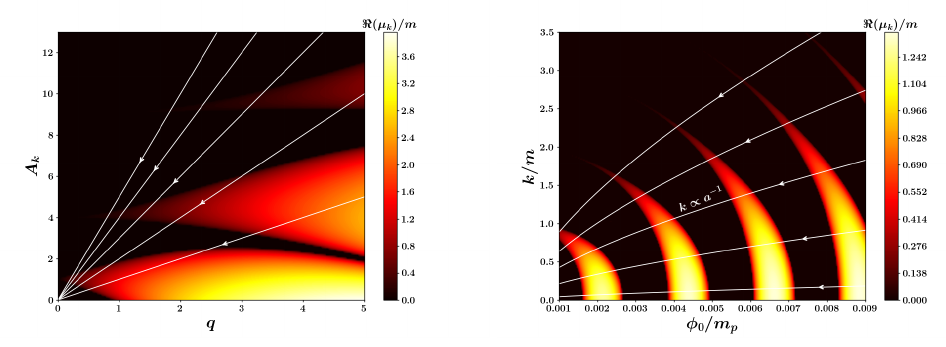
\includegraphics[width=1\linewidth]{Mathieu_apunte2.png}
    \caption{comportamiento de bandas de la ecuación de Mathieu. Se denomina tablas de inestabilidad de Mathieu y dan el valor de los coeficientes de Floquet en función de los parámetros de resonancia $q$ y $A_k$ (izquierda) o $\phi_0$ y $k$ (derecha). Mientras más marrón es la zona más estable es la solución y mientras más amarilla más inestable.}
    \label{fig:Mathieu_apunte2}
\end{figure}

En la Figura \ref{fig:Mathieu_apunte2} podemos ver una tabla de inestabilidad para la ecuación de Mathieu dónde se muestra el valor de la parte real de los coeficientes de Floquet y se puede ver para qué valores de los coeficientes de resonancia tenemos estabilidad. La estabilidad se tiene cuando $\Re \{\mu_q\} = 0$, ya que para éstas tenemos que la amplitud crece exponencialmente por tanto el número de partículas producidas también lo hará.

La densidad de partículas que se generan está dada por la ecuación

\begin{equation}
    n_\chi (k) = \frac{1}{2 \Omega_\chi} \left[ \left| \frac{d \chi_k}{d T} \right|^2 + \Omega_\chi^2 |\chi_k|^2  \right] - \frac{1}{2} \propto e^{2 \mu_k T} 
\end{equation}

\noindent
con $\displaystyle \Omega_\chi = \frac{k^2}{a^2} + g^2 \phi^2$.

Según el comportamiento de la banda en la resonancia paramétrica, podemos encontrarnos con dos tipos de regímenes: \textit{narrow resonance} o \textit{broad resonance}:

\begin{itemize}
    \item El régimen de \textit{narrow resonance} ocurre cuando el parámetro de acoplamiento $q$ es muy pequeño. En este régimen, la amplificación de los modos del campo $\chi$ se concentran en regiones muy estrechas del espacio de momentos. 
    
    Estas bandas de inestabilidad aparecen cuando $A_k \rightarrow n^2$ con $n \in \mathbb{Z}^+$. En estos casos, la banda más relevante es la primera ($n = 1$) ya que es la más ancha dentro de este régimen y corresponde a la producción de dos partículas $\chi$ con $k \approx m$, a partir de la desintegración de dos inflatones. Para valores más altos de $n$, las bandas son cada vez más angostas porque su ancho es proporcional a $q^n$ y representan la desintegración simultánea de $2 n$ inflatones en un par de partículas $\chi$ con $k \simeq n m$. Todo ésto se hace de forma suave. 
    
    Como las interacciones en este régimen son débiles, la frecuencia de los modos $\chi$ permanece prácticamente constante, lo que permite que el inflatón siga oscilando de forma coherente.

    \item El régimen de \textit{broad resonancia} ocurre cuando el parámetro de resonancia $q$ es grande, entonces la amplificación de los modos del campo $\chi$ se concentran en bandas anchas.

    Este tipo de resonancia ocurre en un límite no perturbativo. Y se vuelve más eficiente que el otro régimen de resonancia. Pero las partículas se generan de forma abrupta en vez de en la forma suave que teníamos antes como consecuencia de un cambio no adiabático en la frecuencia del oscilador, este último cambio está dado por

    \begin{equation}
        \left| \frac{d \Omega_\chi}{dT} \right| \geq \Omega^2 (\chi, T) \hspace{2cm} \Longrightarrow \hspace{2cm}  2q |\sin (2T)| \geq \left[ \left( \frac{k}{m} \right)^2 + 4q \sin^2 (T) \right]^{3/2}
    \end{equation}
\end{itemize}

\noindent
\textbf{(2) Backreaction}

Una vez pasado \textit{preheating}, se tiene un \textit{backreaction} dónde las partículas del campo hijo $\chi$ crecen de forma explosiva. Este retroceso se vuelve significativo cuando la densidad de energía de las fluctuaciones se vuelve comparable con la densidad de energía del inflatón, lo que genera una fragmentación del condensado del inflatón. Este fenómeno genera que las oscilaciones coherentes disminuyan haciendo que la producción de partículas $\chi$ también lo haga.

\noindent
\textbf{(3) Scattering and thermalization}

El último estadío de \textit{reheating} es la termalización y la dispersión de las partículas. Durante esta etapa, el remanente del campo inflatón decae de forma perturbativa generando una gran cantidad de otras partículas hijas. Estas partículas a su vez pueden decaer en nuevas partículas y se irán dispersando. Eventualmente todos estos productos termalizarán dando comienzo a la etapa de radiación y luego a BBN.

Hay que tener en cuenta que todo lo que mencionamos acá fue considerando que el universo no se expande, si consideramos la expansión tendremos que de a poco los campos se irán homogeneizando. Y esta expansión podría generar una resonancia estocástica también.